\section{Theorie}
\label{sec:Theorie}
Im vorliegenden Experiment wird die Thermische Elektronenemission untersucht. Dabei werden mit Hilfe des glühelektrischen Effekts freie Elektronen aus einer Metalloberfläche gelöst.
Ziel des Versuches ist es die Temperaturabhängigkeit und die Austrittsarbeit des verwendeten Wolframs zu bestimmen.

Eine Durchführung des Versuches ist nur im Hochvakuum möglich, da die freien Elektronen nicht mit den Gasmolekülen wechselwirken sollen.
Es bietet sich eine Hochvakuumdiode an, welche wie in Abbildung \ref{fig:diode} beschaltet wird.
\begin{figure}
    \centering
    \caption{Beschaltung einer Hochvakuumdiode \cite{v504}}
    \label{fig:diode}
    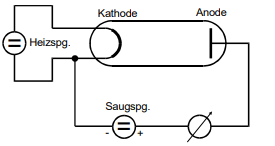
\includegraphics[width = 0.5 \textwidth]{pics/Vakuumdiode.png}
\end{figure}
Das Erhitzen der Kathode erfolgt durch einen starken Heizstrom (ca. $\SI{2.6}{\ampere}$). Durch diesen Heizstrom wird die Kathode auf etwa $\SI{3000}{\kelvin}$ erhitzt, wodurch Elektronen emittiert werden.
Durch eine angelegte Saugspannung werden die Elektronen in Richtung der Anode beschleunigt.

Beim auftragen der Spannung zwischen Kathode und Anode gegen den fließenden Strom, wird eine Kennlinie sichtbar.
Ene typische Kennlinie ist in Abbildung \ref{fig:kennlinie} zu sehen.
\begin{figure}
    \centering
    \caption{Kennlinie einer Hochvakuumdiode \cite{v504}}
    \label{fig:kennlinie}
    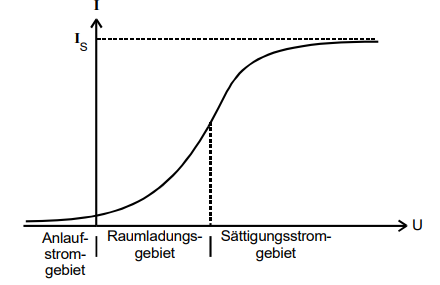
\includegraphics[width = 0.5 \textwidth]{pics/kennlinie.png}
\end{figure}
Die Kennlinie wird in drei Teile unterteilt. 
Der erste Teil ist das Anlaufstromgebiet. In diesem Gebiet ist die Spannung umgepolt, so dass eine Gegenspannung vorliegt.
Es fällt auf, dass für kleine Gegenspannungen auch Elektronen ankommen, da einige dieser Elektronen genug kinetische Energie haben um den Potentialunterschied zu überwinden.
Dies ist möglich da die ausgelösten Elektronen eine statistisch verteilte Bewegungsenergie aufweisen. Eine Abhängigkeit der Stromdichte von der gegenspannung ist gegeben durch
\begin{equation}
    j(V)=const \exp\left(-\frac{e_0 V}{k_\text{B} T}\right) \, .
    \label{eqn:anlauf}
\end{equation}

Das zweite Gebiet wird Raumladungsgebiet genannt. In diesem Gebiet erreichen nicht alle Elektronen die Anode aufgrund der nicht gleichmäßigen Raumladungsdichte.
Diese entsteht durch die beschleunigte Bewegung der Elektronen im Elektrischen Feld. Einige Elektronen werden so mit nicht von dem Anodenfeld erfasst, so dass einige Feldlinien an den Raumladungselektronen vor der Kathode enden.
Die Raumladungsdichte nimmt in Richtung der Anode ab, dies lässt sich anhand der Gleichung \eqref{eqn:dichte} erkennen.
\begin{equation}
    j=- \rho V
    \label{eqn:dichte}
\end{equation}
Anstelle des Ohmschen Gesetzes gilt in diesem Bereich das Langmuir-Schottkysche Raumladungsgesetz:
\begin{equation}
    j=4/9 \, \epsilon_0\, \sqrt{2 \frac{e_0}{m_0}} \, \frac{V^{\frac{3}{2}}}{a^2}
    \label{eqn:drei halbe}
\end{equation}
Die Propornalität $j \sim V^{\frac{3}{2}}$ ist nur eine Näherung aufgrund der Herleitung.

Der dritte Bereich ist das Sättigungsstromgebiet. Der Sättigungsstrom ist erreicht wenn alle Elektronen die Anode erreichen. Gegeben ist die Grenzstromdichte durch die Richardson Gleichung
\begin{equation}
    j_{\text{s}}(T)=4 \pi\, \frac{e_0 m_0 k_\text{b}^2}{h^3}\, T^2 \exp \left(\frac{-e_0 \phi}{k_\text{b} T}\right) \, .
    \label{eqn:richard}
\end{equation}
Die Stromladungsdichte ist nur noch von der Temperatur und der Austrittsarbeit $W_\text{A}=e_0 \phi$ abhängig.

Aus der Leistungsbilanz und der Energieerhaltung folgt die Gleichung:
\begin{equation}
    T=\sqrt[4]{\frac{I_\text{f} U_\text{f}- N_\text{WL}}{f \eta \sigma}} \, .
    \label{eqn:ein viertel}
\end{equation}
Mit dieser lässt sich die Temperatur ermitteln.
Dabei ist $\sigma$ die Sefan-Boltzmannsche Strahlungskonstante, f die emittierende Kathodenoberfläche und $\eta=0.28$ der Emissionsgrad der Oberfäche.